\documentclass[12pt]{extarticle}
\usepackage{phys460}

\title{PHYS460 - Homework 4}
\author{John Hurst}
\date{October 2024}

\begin{document}
\maketitle

%%%%%%%%%%%%%%%%%%%%%%%%%%%%%%%%%%%%%%%%%%%%%%%%%%%%%%%%%%%%%%%%%%%%%%%%%%%%%%%%%%%%%%%%%%%%%%%%%%%%
\question{A2.2}{Prove Lagrange's theorem: if $H$ is a subgroup of a finite group $G$, then the order of $H$ divides the order of $G$.}

Let $m=|H|$, so that $H = \{h_1, h_2, \ldots, h_m\}$.

Choose $g_1 \in G \setminus H$, and define
\[
G_1 = \{g_1h_1, g_1h_2, \ldots, g_1h_m\}.
\]
Then:
\begin{itemize}
\item $G_1 \cap H = \emptyset$, for if $g_1h_i = h_j$ for some $i$ and $j$, then $h_jh_i^{-1}= g_1 \in H$.
\item The elements of $G_1$ are distinct, for if $g_1h_i = g_1h_j$ for some $i$ and $j$, then $\inv{g_1}g_1h_i = h_i = \inv{g_1}g_1h_j = h_j$.
\item Therefore, $|G_1| = m$.
\end{itemize}

If $G\setminus G_1$ is not empty, choose $g_2 \in G\setminus G_1 \setminus H$ and define $G_2$ again as above.

Continue this process until $G \setminus (G_1 \cup G_2 \cup G_3 \cup \ldots \cup G_k) = H$, and there are no more elements to choose.
Then
\begin{align*}
G & = G_1 \cup G_2 \cup \ldots \cup G_k \cup H \\
|G| & = |G_1| + |G_2| + \ldots + |G_k| + m \\
& = (k+1)m \\
& = (k+1)|H|.
\end{align*}

% %%%%%%%%%%%%%%%%%%%%%%%%%%%%%%%%%%%%%%%%%%%%%%%%%%%%%%%%%%%%%%%%%%%%%%%%%%%%%%%%%%%%%%%%%%%%%%%%%%%%
% \question{A2.13}{Show that every irreducible Abelian matrix group is one-dimensional.}

%%%%%%%%%%%%%%%%%%%%%%%%%%%%%%%%%%%%%%%%%%%%%%%%%%%%%%%%%%%%%%%%%%%%%%%%%%%%%%%%%%%%%%%%%%%%%%%%%%%%
\question{A2.7}{Show that every subgroup of a cyclic group is cyclic.}

Let $G$ be a cyclic group with generator $a$, such that $G = \langle a \rangle$.

Let $H$ be a subgroup of $G$.

Let $m=\min\{n: n>0, a^n \in H\}$.

If $m=1$, then $a\in H$ and $H = G$, and is therefore cyclic.

Suppose $m>1$.

Let $b = a^m$.

Consider any $h \in H$. Because $h\in G$, we know that $h=a^k$ for some $k$.

Let
\begin{align*}
d & = \floor{k/m} && \expl{Aka ``$k \text{ div } m$''} \\
r & = k \mod m.
\end{align*}

Then $k = md + r$.

Therefore
\begin{align*}
h & = a^k \\
& = a^{md+r} \\
& = (a^m)^d a^r \\
& = b^d a^r.
\end{align*}

If $m$ does not divide $k$, then $0<r<m$ and $a^r \in H$.
But this is a contradiction because $m$ is the smallest positive integer such that $a^m \in H$.

Therefore $m$ divides $k$, and $h = b^d$ for some $d$.
Therefore $H = \langle b \rangle$, and is cyclic.


%%%%%%%%%%%%%%%%%%%%%%%%%%%%%%%%%%%%%%%%%%%%%%%%%%%%%%%%%%%%%%%%%%%%%%%%%%%%%%%%%%%%%%%%%%%%%%%%%%%%
\question{A2.16}{$S_3$ is the group of permutations of three elements.
Suppose we order these as mapping 123 to 123; 231; 312; 213; 132, and 321, respectively.
Show that there exist two one-dimensional irreducible representations of $S_3$, one of which is trivial,
and the other of which is 1, 1, 1, -1, -1, -1, corresponding in order to the six permutations given earlier.
Also show that there exists a two-dimensional irreducible representation, with the matrices
\begin{align*}
\begin{pmatrix}
    1 & 0 \\
    0 & 1
\end{pmatrix}, &&
\frac{1}{2}
\begin{pmatrix}
    -1 & -\sqrt{3} \\
    \sqrt{3} & -1
\end{pmatrix}, &&
\frac{1}{2}
\begin{pmatrix}
    -1 & \sqrt{3} \\
    -\sqrt{3} & -1
\end{pmatrix}, \\
\begin{pmatrix}
    -1 & 0 \\
    0 & 1
\end{pmatrix}, &&
\frac{1}{2}
\begin{pmatrix}
    1 & \sqrt{3} \\
    \sqrt{3} & -1
\end{pmatrix}, &&
\frac{1}{2}
\begin{pmatrix}
    1 & -\sqrt{3} \\
    -\sqrt{3} & -1
\end{pmatrix}.
\end{align*}
Verify that the representations are orthogonal.
}

The trivial representation is the number 1, which is a valid one-dimensional matrix representation of any group.
It is a representation because if for $g\in G$, $\chi(g) = 1$, then $g_1g_2 = g_3 \implies \chi(g_1)\chi(g_2) = \chi(g_3) = 1$ is tautological.
It is irreducible by definition because it is one-dimensional.

The representation 1, 1, 1, -1, -1, -1 is also one-dimensional.
The permutations 123, 231 and 312 preserve the cyclic ordering. The permutations 213, 132 and 321 reverse the cyclic ordering.
These correspond to 1 and -1 respectively, and the representation mapping is equivalent to:
\[
\chi(g) = \begin{cases}
1 & \text{if $g$ preserves the cyclic ordering} \\
-1 & \text{if $g$ reverses the cyclic ordering}.
\end{cases}
\]

The group of permutations of three elements can be represented by rotations and reflections on the vertices of an equilateral triangle, as shown in Table \ref{tab:permutations}.
\begin{table}[h!]
\centering
\begin{tabular}{ccc}
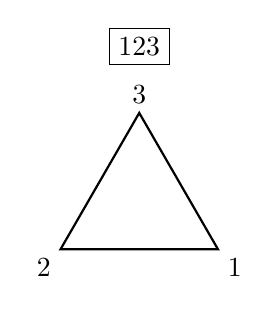
\begin{tikzpicture}
\node[draw] at (0,2) {123};
\coordinate (A) at (0,1.1547);
\coordinate (B) at (-1,-0.5774);
\coordinate (C) at (1,-0.5774);
\draw[thick] (A) -- (B) -- (C) -- cycle;
\node[above] at (A) {3};
\node[below left] at (B) {2};
\node[below right] at (C) {1};
\end{tikzpicture}
&
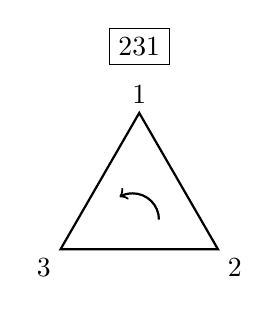
\begin{tikzpicture}
\node[draw] at (0,2) {231};
\coordinate (A) at (0,1.1547);
\coordinate (B) at (-1,-0.5774);
\coordinate (C) at (1,-0.5774);
\draw[thick] (A) -- (B) -- (C) -- cycle;
\node[above] at (A) {1};
\node[below left] at (B) {3};
\node[below right] at (C) {2};
\draw[->,thick] (0.25,-0.2) arc[start angle=0,end angle=120,radius=1/3];
\end{tikzpicture}
&
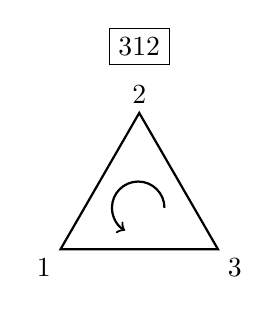
\begin{tikzpicture}
\node[draw] at (0,2) {312};
\coordinate (A) at (0,1.1547);
\coordinate (B) at (-1,-0.5774);
\coordinate (C) at (1,-0.5774);
\draw[thick] (A) -- (B) -- (C) -- cycle;
\node[above] at (A) {2};
\node[below left] at (B) {1};
\node[below right] at (C) {3};
\draw[->,thick] (0.32,-0.05) arc[start angle=0,end angle=240,radius=1/3];
\end{tikzpicture}
\\
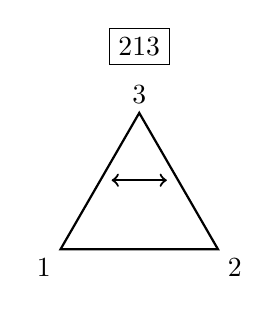
\begin{tikzpicture}
\node[draw] at (0,2) {213};
\coordinate (A) at (0,1.1547);
\coordinate (B) at (-1,-0.5774);
\coordinate (C) at (1,-0.5774);
\draw[thick] (A) -- (B) -- (C) -- cycle;
\node[above] at (A) {3};
\node[below left] at (B) {1};
\node[below right] at (C) {2};
\draw[<->,thick] (0.35,0.3) -- (-0.35,0.3);
\end{tikzpicture}
&
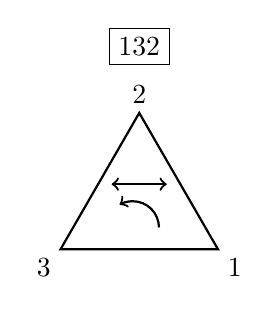
\begin{tikzpicture}
\node[draw] at (0,2) {132};
\coordinate (A) at (0,1.1547);
\coordinate (B) at (-1,-0.5774);
\coordinate (C) at (1,-0.5774);
\draw[thick] (A) -- (B) -- (C) -- cycle;
\node[above] at (A) {2};
\node[below left] at (B) {3};
\node[below right] at (C) {1};
\draw[<->,thick] (0.35,0.25) -- (-0.35,0.25);
\draw[->,thick] (0.25,-0.3) arc[start angle=0,end angle=120,radius=1/3];
\end{tikzpicture}
&
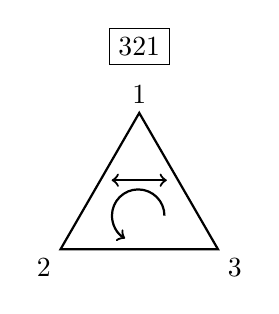
\begin{tikzpicture}
\node[draw] at (0,2) {321};
\coordinate (A) at (0,1.1547);
\coordinate (B) at (-1,-0.5774);
\coordinate (C) at (1,-0.5774);
\draw[thick] (A) -- (B) -- (C) -- cycle;
\node[above] at (A) {1};
\node[below left] at (B) {2};
\node[below right] at (C) {3};
\draw[<->,thick] (0.35,0.3) -- (-0.35,0.3);
\draw[->,thick] (0.32,-0.15) arc[start angle=0,end angle=240,radius=1/3];
\end{tikzpicture}
\end{tabular}
\caption{Permutations of three elements.}
\label{tab:permutations}
\end{table}

\newpage

Let
\begin{align*}
\text{R}(\theta) & = \begin{pmatrix} \cos(\theta) & -\sin(\theta) \\ \sin(\theta) & \cos(\theta) \end{pmatrix} && \expl{2D rotation by $\theta$} \\
\text{M} & = \begin{pmatrix} -1 & 0 \\ 0 & 1 \end{pmatrix} && \expl{reflection about the $y$-axis}.
\end{align*}

Then the permutations can be represented as:

\begin{align*}
\chi(123) & = \text{R}(0)
&& = \begin{pmatrix} \cos(0) & -\sin(0) \\ \sin(0) & \cos(0) \end{pmatrix}
&& = \begin{pmatrix} 1 & 0 \\  0 & 1 \end{pmatrix} \\
\chi(231) & = \text{R}\left(\frac{2\pi}{3}\right)
&& = \begin{pmatrix} \cos(\frac{2\pi}{3}) & -\sin(\frac{2\pi}{3}) \\ \sin(\frac{2\pi}{3}) & \cos(\frac{2\pi}{3}) \end{pmatrix}
&& = \frac{1}{2} \begin{pmatrix} -1 & -\sqrt{3} \\ \sqrt{3} & -1 \end{pmatrix} \\
\chi(312) & = \text{R}\left(\frac{4\pi}{3}\right)
&& = \begin{pmatrix} \cos(\frac{4\pi}{3}) & -\sin(\frac{4\pi}{3}) \\ \sin(\frac{4\pi}{3}) & \cos(\frac{4\pi}{3}) \end{pmatrix}
&& = \frac{1}{2} \begin{pmatrix} -1 & \sqrt{3} \\ -\sqrt{3} & -1 \end{pmatrix} \\
\chi(213) & = \text{R}(0) \cdot \text{M}
&& = \begin{pmatrix} \cos(0) & -\sin(0) \\ \sin(0) & \cos(0) \end{pmatrix} \begin{pmatrix}-1 & 0 \\ 0 & 1\end{pmatrix}
&& = \begin{pmatrix} -1 & 0 \\ 0 & 1 \end{pmatrix}\\
\chi(132) & = \text{R}\left(\frac{2\pi}{3}\right) \cdot \text{M}
&& = \begin{pmatrix} \cos(\frac{2\pi}{3}) & -\sin(\frac{2\pi}{3}) \\ \sin(\frac{2\pi}{3}) & \cos(\frac{2\pi}{3}) \end{pmatrix} \begin{pmatrix}-1 & 0 \\ 0 & 1\end{pmatrix}
&& = \frac{1}{2} \begin{pmatrix} 1 & -\sqrt{3} \\ -\sqrt{3} & -1 \end{pmatrix} \\
\chi(321) & = \text{R}\left(\frac{4\pi}{3}\right) \cdot \text{M}
&& = \begin{pmatrix} \cos(\frac{4\pi}{3}) & -\sin(\frac{4\pi}{3}) \\ \sin(\frac{4\pi}{3}) & \cos(\frac{4\pi}{3}) \end{pmatrix} \begin{pmatrix}-1 & 0 \\ 0 & 1\end{pmatrix}
&& = \frac{1}{2} \begin{pmatrix} 1 & \sqrt{3} \\ \sqrt{3} & -1 \end{pmatrix}
\end{align*}

Note: I got the same matrices as in the Nielsen and Chuang exercise, but in a slightly different order.
I could not get the representation to align when following their order.
Either I have missed something, or is it possible there is a mistake in the book?
I checked for errata and there are some listed, but all for much older printings and nothing relating to this exercise.

Let's verify that this mapping is a representation, i.e. that $g_ig_j = g_k \implies \chi(g_i)\chi(g_j) = \chi(g_k)$.
Table \ref{tab:permutationproducts} shows the product of each pair of permutations.
\begin{table}[h!]
    \centering
    \begin{footnotesize}
        \begin{tabular}{c|c|c|c|c|c|c}
            & $g_1=123$ & $g_2=231$ & $g_3=312$ & $g_4=213$ & $g_5=132$ & $g_6=321$ \\
            \hline
            $g_1=123$ & $123=g_1$ & $231=g_2$ & $312=g_3$ & $213=g_4$ & $132=g_5$ & $321=g_6$ \\
            $g_2=231$ & $231=g_2$ & $312=g_3$ & $123=g_1$ & $132=g_5$ & $321=g_6$ & $213=g_4$ \\
            $g_3=312$ & $312=g_3$ & $123=g_1$ & $231=g_2$ & $321=g_6$ & $213=g_4$ & $132=g_5$ \\
            $g_4=213$ & $213=g_4$ & $321=g_6$ & $132=g_5$ & $123=g_1$ & $312=g_3$ & $231=g_2$ \\
            $g_5=132$ & $132=g_5$ & $213=g_4$ & $321=g_6$ & $231=g_2$ & $123=g_1$ & $312=g_3$ \\
            $g_6=321$ & $321=g_6$ & $132=g_5$ & $213=g_4$ & $312=g_3$ & $231=g_2$ & $123=g_1$ \\
        \end{tabular}
    \end{footnotesize}
    \caption{Product of each pair of $g_1, \ldots, g_6$.}
    \label{tab:permutationproducts}
\end{table}

Table \ref{tab:representationproducts} shows the product of each pair of representations $\chi(g_1), \ldots, \chi(g_6)$.
\begin{table}[h!]
    \centering
\begin{footnotesize}
    \begin{tabular}{c|c|c|c|c|c|c}
        & $\text{R}(0)$ & $\text{R}\left(\frac{2\pi}{3}\right)$ & $\text{R}\left(\frac{4\pi}{3}\right)$ & $\text{R}\left(0\right)\cdot\text{M}$ & $\text{R}\left(\frac{2\pi}{3}\right)\cdot\text{M}$ & $\text{R}\left(\frac{4\pi}{3}\right)\cdot\text{M}$ \\
        \hline
        $\text{R}\left(0\right)$                           & $\text{R}\left(0\right)$ & $\text{R}\left(\frac{2\pi}{3}\right)$ & $\text{R}\left(\frac{4\pi}{3}\right)$ & $\text{R}\left(0\right)\cdot\text{M}$ & $\text{R}\left(\frac{2\pi}{3}\right)\cdot\text{M}$ & $\text{R}\left(\frac{4\pi}{3}\right)\cdot\text{M}$ \\
        $\text{R}\left(\frac{2\pi}{3}\right)$              & $\text{R}\left(\frac{2\pi}{3}\right)$ & $\text{R}\left(\frac{4\pi}{3}\right)$ & $\text{R}\left(0\right)$ & $\text{R}\left(\frac{2\pi}{3}\right)\cdot\text{M}$ & $\text{R}\left(\frac{4\pi}{3}\right)\cdot\text{M}$ & $\text{R}\left(0\right)\cdot\text{M}$ \\
        $\text{R}\left(\frac{4\pi}{3}\right)$              & $\text{R}\left(\frac{4\pi}{3}\right)$ & $\text{R}\left(0\right)$ & $\text{R}\left(\frac{2\pi}{3}\right)$ & $\text{R}\left(\frac{4\pi}{3}\right)\cdot\text{M}$ & $\text{R}\left(0\right)\cdot\text{M}$ & $\text{R}\left(\frac{2\pi}{3}\right)\cdot\text{M}$ \\
        $\text{R}\left(0\right)             \cdot\text{M}$ & $\text{R}\left(0\right)\cdot\text{M}$ & $\text{R}\left(\frac{4\pi}{3}\right)\cdot\text{M}$ & $\text{R}\left(\frac{2\pi}{3}\right)\cdot\text{M}$ & $\text{R}(0)$ & $\text{R}\left(\frac{4\pi}{3}\right)$ & $\text{R}\left(\frac{2\pi}{3}\right)$ \\
        $\text{R}\left(\frac{2\pi}{3}\right)\cdot\text{M}$ & $\text{R}\left(\frac{2\pi}{3}\right)\cdot\text{M}$ & $\text{R}\left(0\right)\cdot\text{M}$ & $\text{R}\left(\frac{4\pi}{3}\right)\cdot\text{M}$ & $\text{R}\left(\frac{2\pi}{3}\right)$ & $\text{R}\left(0\right)$ & $\text{R}\left(\frac{4\pi}{3}\right)$ \\
        $\text{R}\left(\frac{4\pi}{3}\right)\cdot\text{M}$ & $\text{R}\left(\frac{4\pi}{3}\right)\cdot\text{M}$ & $\text{R}\left(\frac{2\pi}{3}\right)\cdot\text{M}$ & $\text{R}\left(0\right)\cdot\text{M}$ & $\text{R}\left(\frac{4\pi}{3}\right)$ & $\text{R}\left(\frac{2\pi}{3}\right)$ & $\text{R}\left(0\right)$ \\
    \end{tabular}
\end{footnotesize}
\caption{Product of each pair of $\chi(g_1), \ldots, \chi(g_6)$.}
\label{tab:representationproducts}
\end{table}

Each product in Table \ref{tab:permutationproducts} matches the corresponding product in Table \ref{tab:representationproducts}, so the mapping is a representation.

The representation is irreducible because the rotations cannot be put into an equivalent block-diagonal form. (I don't know how to prove this.)

To ``verify'' that the representations are orthogonal, it sounds as if the question wants me to plug in values and verify the orthogonality relation:
\[
\sum_{g\in G} \left[\rho^p(g)\right]_{ij}^{-1} \left[\rho^q(g)\right]_{kl} = \frac{|G|}{d_p} \delta_{il} \delta_{jk} \delta_{pq},
\]
for all relevant $p$, $q$, $i$, $j$, $k$, and $l$.

I could not see an obvious way to do this that was not extremely tedious, so I have programmed it in Mathematica, and included the notebook in the submission.

% %%%%%%%%%%%%%%%%%%%%%%%%%%%%%%%%%%%%%%%%%%%%%%%%%%%%%%%%%%%%%%%%%%%%%%%%%%%%%%%%%%%%%%%%%%%%%%%%%%%%
% \question{A2.24}{Using the results of exercise A2.16, construct the Fourier transform over $S_3$ and express it as a 6x6 unitary matrix.}

%%%%%%%%%%%%%%%%%%%%%%%%%%%%%%%%%%%%%%%%%%%%%%%%%%%%%%%%%%%%%%%%%%%%%%%%%%%%%%%%%%%%%%%%%%%%%%%%%%%%
\question{10.46}{Show that the stabilizer for the three qubit phase flip code is generated by $X_1X_2$ and $X_2X_3$.}

The subgroup $S\subset G_3$ given by $S = \{I, X_1X_2, X_2X_3, X_3X_1\}$ is generated by $X_1X_2$ and $X_2X_3$,
because $X_1, X_2, X_3$ commute, and:
\begin{align*}
X_1X_2 \cdot X_2X_3 & = X_1X_3 \\
X_1X_2 \cdot X_1X_2 & = X_2X_3 \cdot X_2X_3 = I \\
\end{align*}

The subspace fixed by $X_1X_2$ is spanned by these vectors:
\begin{align*}
u_1 & = \ket{000} + \ket{110} \\
u_2 & = \ket{001} + \ket{111} \\
u_3 & = \ket{010} + \ket{100} \\
u_4 & = \ket{011} + \ket{101} \\
\end{align*}

The subspace fixed by $X_2X_3$ is spanned by these vectors:
\begin{align*}
v_1 & = \ket{000} + \ket{011} \\
v_2 & = \ket{001} + \ket{010} \\
v_3 & = \ket{100} + \ket{111} \\
v_4 & = \ket{101} + \ket{110} \\
\end{align*}

For a vector $w$ in the intersection of these subspaces, we have:
\begin{align*}
w & = a u_1 + b u_2 + c u_3 + d u_4 \\
  & = e v_1 + f v_2 + g v_3 + h v_4. \\
\end{align*}
That is,
\begin{align*}
w & = a (\ket{000} + \ket{110}) + b (\ket{001} + \ket{111}) + c (\ket{010} + \ket{100}) + d (\ket{011} + \ket{101}) \\
  & = e (\ket{000} + \ket{011}) + f (\ket{001} + \ket{010}) + g (\ket{100} + \ket{111}) + h (\ket{101} + \ket{110}). \\
\end{align*}
So that:
\begin{align*}
a & = e = d = h = a, \\
b & = f = c = g = b, \\
\end{align*}
and:
\begin{align*}
w & = a \left( \ket{000} + \ket{110} + \ket{011} + \ket{101} \right) + b \left( \ket{001} + \ket{111} + \ket{010} + \ket{100} \right).
\end{align*}
Therefore, the intersection of the subspaces is spanned by:
\[
\ket{000} + \ket{110} + \ket{011} + \ket{101} + \ket{001} + \ket{111} + \ket{010} + \ket{100}
\]
and
\[
\ket{000} + \ket{110} + \ket{011} + \ket{101} - \ket{001} - \ket{111} - \ket{010} - \ket{100},
\]
which are the two codewords of the three qubit phase flip code.

Note that Proposition 10.5 with $S=\langle X_1X_2, X_2X_3 \rangle$, $n=3$, and $k=1$ also
requires that $V_S$ is a $2^k$ = 2-dimensional vector space.

%%%%%%%%%%%%%%%%%%%%%%%%%%%%%%%%%%%%%%%%%%%%%%%%%%%%%%%%%%%%%%%%%%%%%%%%%%%%%%%%%%%%%%%%%%%%%%%%%%%%
\question{10.47}{Verify that the generators of Table \ref{tab:stabilizers} generate the two codewords given by
\begin{align*}
\ket{0} \rightarrow \ket{0_L} & \equiv \frac{(\ket{000} + \ket{111})(\ket{000} + \ket{111})(\ket{000} + \ket{111})}{2\sqrt{2}} \\
\ket{1} \rightarrow \ket{1_L} & \equiv \frac{(\ket{000} - \ket{111})(\ket{000} - \ket{111})(\ket{000} - \ket{111})}{2\sqrt{2}}
\end{align*}

\begin{table}[h!]
\centering
\qtext{
\begin{tabular}{|c|c|}
\hline
Name & Operator \\
\hline
$g_1$          & $Z \; Z \; I \; I \; I \; I \; I \; I \; I$ \\
$g_2$          & $I \; Z \; Z \; I \; I \; I \; I \; I \; I$ \\
$g_3$          & $I \; I \; I \; Z \; Z \; I \; I \; I \; I$ \\
$g_4$          & $I \; I \; I \; I \; Z \; Z \; I \; I \; I$ \\
$g_5$          & $I \; I \; I \; I \; I \; I \; Z \; Z \; I$ \\
$g_6$          & $I \; I \; I \; I \; I \; I \; I \; Z \; Z$ \\
$g_7$          & $X \; X \; X \; X \; X \; X \; I \; I \; I$ \\
$g_8$          & $I \; I \; I \; X \; X \; X \; X \; X \; X$ \\
$\overline{Z}$ & $X \; X \; X \; X \; X \; X \; X \; X \; X$ \\
$\overline{X}$ & $Z \; Z \; Z \; Z \; Z \; Z \; Z \; Z \; Z$ \\
\hline
\end{tabular}
}
\caption{\qtext{Generators for the Shor code, and the logical $Z$ and $X$ operators.}}
\label{tab:stabilizers}
\end{table}
}

The dimensionalities of the subspaces fixed by these generators are much larger than the ones in the previous question,
so is not practical to write out explicit expressions for the spanning vectors.
Instead, I will provide a more informal argument.

$g_1$ fixes vectors having the form $\ket{00.......}$ and $\ket{11.......}$, i.e. vectors where the first two qubits are the same, but the rest are arbitrary.
$g_2$ fixes vectors where the second and third qubits are the same, and the rest are arbitrary.
Taken together, the intersection of the spaces fixed by these two generators are vectors having all the first three qubits the same, and the rest arbitrary.

Similarly, $g_3$ and $g_4$ fix vectors where the middle three qubits are the same, and the rest are arbitrary,
and $g_5$ and $g_6$ fix vectors where the last three qubits are the same, and the rest are arbitrary.

The intersection of the spaces fixed by these three pairs of generators are vectors where all the qubits
in each of the three triplets are the same, i.e. vectors of the form $\ket{aaabbbccc}$.
% The vectors fixed by $g_7$ are those of the form
% \[
% \ket{b_1b_2b_3b_4b_5b_6b_7b_8b_9} + \ket{\bar{b_1}\bar{b_2}\bar{b_3}\bar{b_4}\bar{b_5}\bar{b_6}b_7b_8b_9},
% \]
% where $b_i$ are arbitrary, and $\bar{b_i}$ are the negations of the $b_i$.
% The vectors fixed by $g_8$ are those of the form
% \[
% \ket{b_1b_2b_3b_4b_5b_6b_7b_8b_9} + \ket{b_1b_2b_3\bar{b_4}\bar{b_5}\bar{b_6}\bar{b_7}\bar{b_8}\bar{b_9}}.
% \]
% And the vectors fixed by $g_7g_8 = X_1X_2X_3X_7X_8X_9$  are those of the form
% \[
% \ket{b_1b_2b_3b_4b_5b_6b_7b_8b_9} + \ket{\bar{b_1}\bar{b_2}\bar{b_3}b_4b_5b_6\bar{b_7}\bar{b_8}\bar{b_9}}.
% \]

We notice that the remaining two generators
\begin{align*}
g_7 & = X_1X_2X_3X_4X_5X_6 \\
g_8 & = X_4X_5X_6X_7X_8X_9
\end{align*}

are completely analgous to $X_1X_2$ and $X_2X_3$ in the previous question,
with $\ket{aaabbbccc}$ in place of $\ket{abc}$.

Therefore the codewords generated by $g_1\ldots g_8$ are:

\begin{multline*}
\ket{000000000} + \ket{111111000} + \ket{000111111} + \ket{111000111} + \\
\ket{000000111} + \ket{111111111} + \ket{000111000} + \ket{111000000}
\end{multline*}
and
\begin{multline*}
\ket{000000000} + \ket{111111000} + \ket{000111111} + \ket{111000111} - \\
\ket{000000111} - \ket{111111111} - \ket{000111000} - \ket{111000000}
\end{multline*}
or
\[
(\ket{000} + \ket{111})(\ket{000} + \ket{111})(\ket{000} + \ket{111})
\]
and
\[
(\ket{000} - \ket{111})(\ket{000} - \ket{111})(\ket{000} - \ket{111}).
\]

%%%%%%%%%%%%%%%%%%%%%%%%%%%%%%%%%%%%%%%%%%%%%%%%%%%%%%%%%%%%%%%%%%%%%%%%%%%%%%%%%%%%%%%%%%%%%%%%%%%%
\question{10.48}{Show that the operations
\begin{align*}
    \overline{Z} & = X_1X_2X_3X_4X_5X_6X_7X_8X_9 \\
    \text{and}\quad \overline{X} & = Z_1Z_2Z_3Z_4Z_5Z_6Z_7Z_8Z_9
\end{align*}
act as logical $Z$ and $X$ operators
on a Shor-coded qubit.
That is, show that this $\overline{Z}$ is independent of and commutes with the generators of the Shor code,
and that $\overline{X}$ is independent of and commutes with the generators of the Shor code,
and anti-commutes with $\overline{Z}$.}

The check matrix representation of Table \ref{tab:stabilizers}, including the eight generators and the logical $Z$ and $X$ operators, is:
\[
\left[
\begin{array}{ccccccccc|ccccccccc}
    0 & 0 & 0 & 0 & 0 & 0 & 0 & 0 & 0  &  1 & 1 & 0 & 0 & 0 & 0 & 0 & 0 & 0 \\
    0 & 0 & 0 & 0 & 0 & 0 & 0 & 0 & 0  &  0 & 1 & 1 & 0 & 0 & 0 & 0 & 0 & 0 \\
    0 & 0 & 0 & 0 & 0 & 0 & 0 & 0 & 0  &  0 & 0 & 0 & 1 & 1 & 0 & 0 & 0 & 0 \\
    0 & 0 & 0 & 0 & 0 & 0 & 0 & 0 & 0  &  0 & 0 & 0 & 0 & 1 & 1 & 0 & 0 & 0 \\
    0 & 0 & 0 & 0 & 0 & 0 & 0 & 0 & 0  &  0 & 0 & 0 & 0 & 0 & 0 & 1 & 1 & 0 \\
    0 & 0 & 0 & 0 & 0 & 0 & 0 & 0 & 0  &  0 & 0 & 0 & 0 & 0 & 0 & 0 & 1 & 1 \\
    1 & 1 & 1 & 1 & 1 & 1 & 0 & 0 & 0  &  0 & 0 & 0 & 0 & 0 & 0 & 0 & 0 & 0 \\
    0 & 0 & 0 & 1 & 1 & 1 & 1 & 1 & 1  &  0 & 0 & 0 & 0 & 0 & 0 & 0 & 0 & 0 \\
    1 & 1 & 1 & 1 & 1 & 1 & 1 & 1 & 1  &  0 & 0 & 0 & 0 & 0 & 0 & 0 & 0 & 0 \\
    0 & 0 & 0 & 0 & 0 & 0 & 0 & 0 & 0  &  1 & 1 & 1 & 1 & 1 & 1 & 1 & 1 & 1 \\
\end{array}
\right].
\]
It is obvious from this that the last two rows, for the two logical operators, are linearly independent of the rows for the generators,
meaning that the logical operators are independent of the generators.

It is also obvious that $\overline{Z}$ anticommutes with $\overline{X}$, i.e. $\overline{Z}\overline{X} = -\overline{X}\overline{Z}$,
because $XZ = -ZX$.

The reason that the logical operators commute with the generators is the same reason that the generators commute with one another.
For any pair $(\overline{X},g_k)$ or $(\overline{Z},g_k)$, there are always an even number of positions in which there is an $X$ in one of the elements and a $Z$ in the other,
meaning that there is an even number of anticommuting pairs, and the -1 factors cancel out.

% \printbibliography
% \addcontentsline{toc}{section}{References}

\end{document}
